
\section{Машинное обучение}

\subsection{Понятие искусственной нейронной сети}

Машинное обучение (Machine Learning) – раздел исследований в сфере ИИ, в основе которых лежат методы разработки систем способных к обучению. Алгоритмы машинного обучения эффективно себя показывают в задачах, в которых требуется у заранее подготовленных (обучающих) данных определить общие признаки и по ним идентифицировать новые данные. В проектировании таких, обучающихся, систем часто применяют искуственные нейронные сети. 

Искусственная нейронная сеть (ИНС) – компьютерная модель, в основе которой лежат принципы работы биологической нейронной сети - совокупности связанных между собой нервных клеток - нейронов. Каждый нейрон имеет набор входных связей - синапсов, по которым он получает информацию, представленную в виде импульсов, от других нейронов. По полученным данным нейрон формирует своё состояние и, с помощью аксона, сообщает его другим нейронам, обеспечивая функционирование системы. В процессе формирования системы одни нейронные связи укрепляются, а другие ослабляются, обеспечивая обучаемость сети.
\addimghere{biological-neuron}{0.5}{Типичная структура биологического нейрона}{biological-neuron}

Искусственный нейрон представляет собой упрощенную модель биологического нейрона. Принцип его работы представлен на рисунке \ref{simple-neuron}. Сначала нейрон получает n-мерные вектор входных значений $X=(x_{1},...,x_{n})$ и вектор весов $W=(w_{1},...,w_{n})$, обозначающий <<укрепленность>> межнейронных связей. Вычесляется сумма произведения входных значений и весов $s_j$. Затем к полученному результату применяется \hyperref[sec:activation]{функция активации} ($\varphi$). В некоторых случаях, к сумме прибавляется величина смещения $b_j$.
\begin{figure}[H]
  \centering

  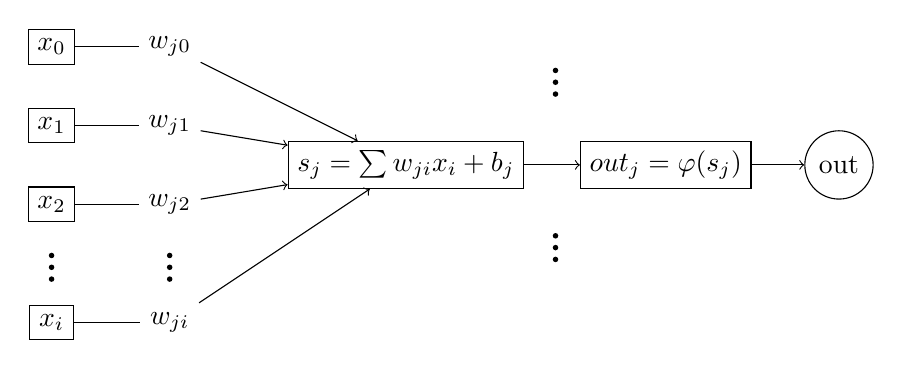
\begin{tikzpicture}
    \tikzstyle{rectangle_style}=[rectangle, draw]
    \tikzstyle{dividedrectangle_style}=[draw, rectangle split, rectangle split parts=2, rotate = 90, minimum height = 15mm, minimum width = 10mm]
    
    % neuron i
    \foreach \x in {0,...,2}
      \draw node at (0, -\x) [rectangle_style] (neuron_i_\x) {$x_\x$};
    \foreach \x in {1,...,3}
      \fill (0, -2.5 - \x*0.15) circle (1pt);
    \draw node at (0, -3.5) [rectangle_style] (neuron_i_3) {$x_i$};
    
    % w_ji
    \foreach \x in {0,...,2}
      \draw node at (1.5, -\x) [] (w_ji_\x) {$w_{j\x}$};
    \draw node at (1.5, -3.5) [] (w_ji_i) {$w_{ji}$};
    \foreach \x in {1,...,3}
      \fill (1.5, -2.5 - \x*0.15) circle (1pt);
    
    % neuron sum
    \draw node at (4.5, -1.5) [rectangle_style] (neuron_sum) {
      $s_j = \sum {w_{ji}x_i+b_j}$
    };
    \draw node at (7.8, -1.5) [rectangle_style] (neuron_act) {
      $out_j = \varphi (s_j)$
    };
    \foreach \x in {1,...,3}
      \fill (6.4, -2.25 - \x*0.15) circle (1pt);
    \foreach \x in {1,...,3}
      \fill (6.4,  - 0.15 - \x*0.15) circle (1pt);
    
    % output
    \node at (10, -1.5) [circle, draw] (output) {out};    

    
    % connect: y_i -> w_ji
    \foreach \i in {0,...,2}
      \path[-] (neuron_i_\i) edge node[] {} (w_ji_\i);
    \path[-] (neuron_i_3) edge node[] {} (w_ji_i);
    
    % connect: w_ji -> neuron j
    \foreach \i in {0,...,2}
      \path[->] (w_ji_\i) edge node[] {} (neuron_sum);
    \path[->] (w_ji_i) edge node[] {} (neuron_sum);
    
     % connect: neuron sum  -> neuron act
     \path[->] (neuron_sum) edge node[above, midway] {$ $} (neuron_act);

    % connect: neuron act -> output
    \path[->] (neuron_act) edge node[above, midway] {$ $} (output);

    
  \end{tikzpicture}
\caption{Схема искусственного нейрона} \label{simple-neuron}
\end{figure}

Множества нейронов формируют слои, слои в свою очередь формируют нейронную сеть. Входной слой получает данные, обрабатывает и передает нейронам скрытого слоя. Аналогично срабатывет каждый последующий слой вплоть до выходного. 

\tikzset{%
every neuron/.style={
  circle,
  draw,
  minimum size=1cm
},
neuron missing/.style={
  draw=none, 
  scale=4,
  text height=0.333cm,
  execute at begin node=\color{black}$\vdots$
},
}
\begin{figure}[H]
  \centering
\begin{tikzpicture}[x=1.5cm, y=1.5cm, >=stealth]

\foreach \m/\l [count=\y] in {1,2,3,missing,4}
\node [every neuron/.try, neuron \m/.try] (input-\m) at (0,2.5-\y) {};

\foreach \m [count=\y] in {1,missing,2}
\node [every neuron/.try, neuron \m/.try ] (hidden-\m) at (2,2-\y*1.25) {};

\foreach \m [count=\y] in {1,missing,2}
\node [every neuron/.try, neuron \m/.try ] (output-\m) at (4,1.5-\y) {};

\foreach \l [count=\i] in {1,2,3,n}
\draw [<-] (input-\i) -- ++(-1,0)
  node [above, midway] {$I_\l$};

\foreach \l [count=\i] in {1,k}
\node [above] at (hidden-\i.north) {$H_\l$};

\foreach \l [count=\i] in {1,p}
\draw [->] (output-\i) -- ++(1,0)
  node [above, midway] {$O_\l$};

\foreach \i in {1,...,4}
\foreach \j in {1,...,2}
  \draw [->] (input-\i) -- (hidden-\j);

\foreach \i in {1,...,2}
\foreach \j in {1,...,2}
  \draw [->] (hidden-\i) -- (output-\j);

\foreach \l [count=\x from 0] in {Входной, Скрытый, Выходной}
\node [align=center, above] at (\x*2,2) {\l \\ слой};
\end{tikzpicture}
\caption{Схема простой нейронной сети} \label{simple-network}
\end{figure}

Нейросети с большим количеством скрытых слоев называется глубокими. Область машинного обучения, в которой используются глубокие нейронные сети называется - глубоким обучением (Deep Learning).     

\subsection{Активационная функция}
\label{sec:activation}
Взвешенная сумма входов представляет собой линейную комбинацию, из чего следует, что независимо от количества слоев, значения выходного слоя зависят только от входов первого слоя. 
Активационная функция нейрона обеспечивает нормализацию посчитанной суммы и нелинейность нейронной сети. Для многих моделей нейронных сетей также требуется, чтобы активационная функция была монотонной и непрерывно-дифференцируемой на всей области определения.

Существует большое количество функций активации. Наиболее распространенные из них представлены в таблице \ref{actvs}.

\pgfplotsset{
  every axis plot/.append style={
    line width=3pt
  }
}

\begin{table}[H]
  \centering
  \caption{Популярные активационные функции}\label{actvs}
  \begin{tabular}{|c|c|c|}
    \hline    
    \hyperlink{name}{Название} & \hyperlink{func}{Функция} & \hyperlink{chart}{Вид}\\
    \hline
    Сигмоидная &  \resizebox{0.2\hsize}{!}{$\sigma(x)=\frac{1}{1+e^{-x}}$}
    & 
    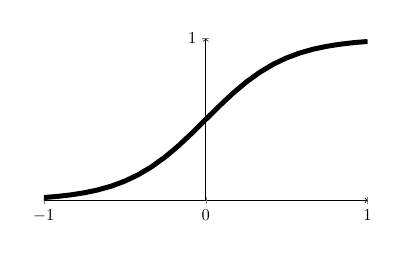
\begin{tikzpicture}[baseline={(0,0.8)}, scale=0.6]      
      \begin{axis}[
        axis equal image,
        axis lines=middle,
        axis line style={->},
        x label style={at={(axis description cs:0.5,-0.1)},anchor=north},
        y label style={at={(axis description cs:-0.1,.5)},rotate=90,      anchor=south},
        extra x ticks=0,
        % extra y ticks=1,
        ymin=0,ymax=1,
        ytick={0, 1},
        xtick={-1, 0, 1}
        ]
        \addplot[domain=-1:1, variable=\x] ({\x},{1/(1+exp(-4*\x))});
      \end{axis}      
    \end{tikzpicture}
   
    \\
    \hline
    Гиперболический тангенс 
    &
    \resizebox{0.2\hsize}{!}{$f(x)=\frac{e^x-e^{-x}}{e^x+e^{-x}}$}
    & 
    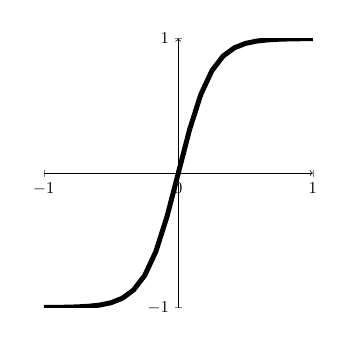
\begin{tikzpicture}[baseline={(0,1.5)},scale=0.6]
      \begin{axis}[
        axis equal image,
        axis lines=middle,
        axis line style={->},
        x label style={at={(axis description cs:0.5,-0.1)},anchor=north},
        y label style={at={(axis description cs:-0.1,.5)},rotate=90,      anchor=south},
         extra x ticks=0,  
        % extra y ticks=1,
        ymin=-1,ymax=1,
        ytick={-1, 0, 1},
        xtick={-1, 0, 1}
        ]
        \addplot[domain=-1:1, variable=\x]({\x},{tanh(4*\x)});
      \end{axis}      
    \end{tikzpicture} 
    \\
    \hline
    ReLU & \resizebox{0.2\hsize}{!}{$f(x) =\begin{cases}
    0, & x<0 \\ 
    x, & x \geq 0.
    \end{cases}$} & 
    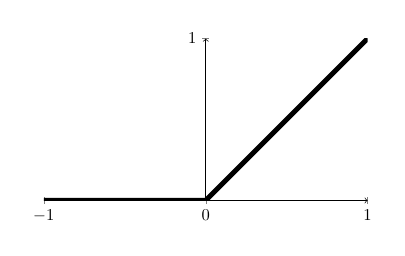
\begin{tikzpicture}[baseline={(0,0.8)},scale=0.6]
      \begin{axis}[
        axis equal image,
        axis lines=middle,
        axis line style={->},
        x label style={at={(axis description cs:0.5,-0.1)},anchor=north},
        y label style={at={(axis description cs:-0.1,.5)},rotate=90,anchor=south},
         extra x ticks=0,  
        % extra y ticks=1,
        ymin=0,ymax=1,
        ytick={0, 1},
        xtick={-1, 0, 1}
        ]
        \addplot[domain=-1:1, variable=\x]({\x},{ifthenelse(\x<0,0,\x)});
      \end{axis}      
    \end{tikzpicture}
    \\
    \hline
  \end{tabular}
\end{table}

\subsection{Обучение нейронных сетей}
Под обучением нейронных сетей подразумевают настройку значений весов связей для эффективного решения поставленной задачи. Изначально, веса устанавливаются случайно. Затем, в процессе прогона через сеть тестовых данных, веса корректируются так, чтобы в конечном итоге сеть выдавала правильные ответы. 

Существует несколько подходов к обучению нейронных сетей:

\subparagraph{Обучение с учителем} \mbox{} \\
Обучение с учителем - это такой тип обучения, в котором сеть получает набор входных данных с заранее известными правильными ответами. Веса корректируются в зависимости от того, правильный ли ответ дала сеть. 

Одним из популярных методов обучения с учителем является алгоритм обратного распространения ошибки \cite{Nielsen2015}, который часто применяется в обучении глубоких нейронных сетей. 

Пусть сеть имеет L слоев, $a^l$, $w_{}^l$, $b^l$ - векторы значений, весов и смещений нейронов на $l$-м слое.. Также имеется N обучающих пар (x,y). 
В процессе обучения циклично происходят следующие итерации: 

\begin{enumerate}
    \item На вход сети подается вектор x из обучающего множества, для каждого слоя вычислить значения: \hfill $z^l = w^la^{l-1}+b^l и a^l = \sigma(z^l)$
    \item Вычислить значение функции стоимости: \hfill $C = \frac{1}{2}\sum_j{(y_j-a_j^L)^2}$
    \item Вычислить значения ошибок выходного слоя: \hfill $\delta_j^L=\frac{\delta C}{\delta a_j^L}\sigma'(z_j^L)$
    \item Вычислить ошибки для каждого предыдущего слоя: \hfill $\delta_j^l=\sum_k{w_{kj}^{l+1} \delta_k^{l+1}\sigma'(z_j^l)}$
    \item Вычислить градиент функции стоимости: \hfill $\frac{\delta C}{\delta w_{jk}^l} = a_k^{l-1} \delta_j^l$ % и $\frac{\delta C}{\delta b_j^l} = \delta_j^l$
    \item Обновить веса связей: \hfill $w_{ij}^l=w_{ij}^l-\mu\frac{\delta C}{\delta w_{jk}^l},\hspace{1em} 0<\mu \leqslant 1$
\end{enumerate}
%%%%%%%%%%%%%%%%%%%%%%%%%%%%%%%%%%%%%%%%%%%%%%%%%%%%%%%%%
% http://neuralnetworksanddeeplearning.com/chap2.html
%%%%%%%%%%%%%%%%%%%%%%%%%%%%%%%%%%%%%%%%%%%%%%%%%%%%%%%%%

\subparagraph{Обучение с подкреплением}\mbox{} \\
 Данный метод подразумевает наличие некоторой окружающей среды в которой действует сеть. Такая среда реагирует на действия модели и подает ей определенные сигналы.  

\subparagraph{Обучение без учителя}\mbox{} \\
Обучение при котором сеть заренее не располагает правильными ответами и самостоятельно ищет общие и отличительные признаки у входных данных. 


\subparagraph{Генетические алгоритмы обучения}\mbox{} \\
 Алгоритмы, имитирующие эволюционные механизмы развития биологической популяции, выступают как альтернатива алгоритму обратного распространения ошибки. Значение произвольного весового коэффициента в нейронной сети называется геном. Гены формируют хромосомы, а хромосомы - популяцию. Дальше, в пределах одного цикла (эпохи) с определенными вероятностями происходит: 
 \begin{itemize}
     \item Cкрещивание хромосом - формирование новой хромосомы из генов двух других
     \item мутация - случайное изменение произвольного гена
     \item приспособление - (хромосомы показавшие худшие результаты уничтожаются из популяции.
 \end{itemize}

+/- ???

\subsection{Сверточные нейронные сети}
Стандартные нейронные сети состоят из полносвязных слоев - слоев, в которых каждый нейрон связан с каждым нейроном следующего слоя, что значительно увеличивает вычислительную сложность системы при увеличении количества нейронов. 
В типовых сверточных нейронных сетях к полносвязным добавляются сверточные и подвыборочные слои. 

Сверточные слои характеризуются использованием матриц весов, называемых фильтрами или ядрами, которые обладают размерностью меньше исходных данных. Такое ядро с определенным шагом проходит по набору входных данных $(I)$ и вычисляет суммы произведений соответствующих значений ячеек и весов, формируя карту признаков $(I * K)$. Один сверточный слой может содержать несколько ядер и соответственно несколько карт признаков.

\begin{figure}[H]
\centering
\begin{tikzpicture}

	\matrix (mtr) [matrix of nodes,row sep=-\pgflinewidth, nodes={draw}]
	{
		0 & 1 & 1 & |[fill=red!30]| 1 & |[fill=red!30]| 0 & |[fill=red!30]| 0 & 0\\
		0 & 0 & 1 & |[fill=red!30]| 1 & |[fill=red!30]| 1 & |[fill=red!30]| 0 & 0\\
		0 & 0 & 0 & |[fill=red!30]| 1 & |[fill=red!30]| 1 & |[fill=red!30]| 1 & 0\\
		0 & 0 & 0 & 1 & 1 & 0 & 0\\
		0 & 0 & 1 & 1 & 0 & 0 & 0\\
		0 & 1 & 1 & 0 & 0 & 0 & 0\\
		1 & 1 & 0 & 0 & 0 & 0 & 0\\
	};

	\draw[very thick, red] (mtr-1-4.north west) rectangle (mtr-3-6.south east);

	\node [below= of mtr-5-4.south] (lm) {$\bf I$};

	\node[right = 0.2em of mtr] (str) {$*$};

	\matrix (K) [right=0.2em of str,matrix of nodes,row sep=-\pgflinewidth, nodes={draw, fill=blue!30}]
	{
		1 & 0 & 1 \\
		0 & 1 & 0 \\
		1 & 0 & 1 \\
	};
	\node [below = of K-3-2.south] (lk) {$\bf K$};

	\node [right = 0.2em of K] (eq) {$=$};

	\matrix (ret) [right=0.2em of eq,matrix of nodes,row sep=-\pgflinewidth, nodes={draw}]
	{
		1 & 4 & 3 & |[fill=green!30]| 4 & 1\\
		1 & 2 & 4 & 3 & 3\\
		1 & 2 & 3 & 4 & 1\\
		1 & 3 & 3 & 1 & 1\\
		3 & 3 & 1 & 1 & 0\\
	};
	\node [below = of ret-4-3.south] (lim) {${\bf I} * {\bf K}$};

	\draw[very thick, green] (ret-1-4.north west) rectangle (ret-1-4.south east);

	\draw[densely dotted, blue, thick] (mtr-1-4.north west) -- (K-1-1.north west);
	\draw[densely dotted, blue, thick] (mtr-3-4.south west) -- (K-3-1.south west);
	\draw[densely dotted, blue, thick] (mtr-1-6.north east) -- (K-1-3.north east);
	\draw[densely dotted, blue, thick] (mtr-3-6.south east) -- (K-3-3.south east);

	\draw[densely dotted, green, thick] (ret-1-4.north west) -- (K-1-1.north west);
	\draw[densely dotted, green, thick] (ret-1-4.south west) -- (K-3-1.south west);
	\draw[densely dotted, green, thick] (ret-1-4.north east) -- (K-1-3.north east);
	\draw[densely dotted, green, thick] (ret-1-4.south east) -- (K-3-3.south east);

	\matrix (K) [right=0.2em of str,matrix of nodes,row sep=-\pgflinewidth, nodes={draw, fill=blue!10}]
	{
		1 & 0 & 1 \\
		0 & 1 & 0 \\
		1 & 0 & 1 \\
	};

	\draw[very thick, blue] (K-1-1.north west) rectangle (K-3-3.south east);

\end{tikzpicture}
\caption{Операция свертки} \label{convolution}
\end{figure}

Так как признаки уже обнаружены, для упрощения дальнейших вычислений можно снизить детализацию входных данных. Это обеспечивает подвыборочный (пулинговый) слой, сжимая карты признаков, полученные от сверточного слоя, что снижает количество параметров, используемых в дальнейших вычислениях сети. 

СНС может иметь несколько пар чередующихся сверточных и подвыборочных слоев. Завершается СНС стандартными полносвязными слоями.  

\subsection{Рекуррентные нейронные сети}
Все вышеуказанные архитектуры нейронных сетей являются статическими - имеют заранее заданные параметры, без возможности их корректирования в процессе работы сети.

???
\clearpage